% !TEX root = ../thesis.tex
\chapter{Features engineering}
\label{capitolo4}
\thispagestyle{empty}

This chapter can be seen as one of the most important of the whole project.

We wouldn't have hit such performances, if it wasn't for feature engineering. We had a large pool of models to pick for our purpose,  and we tried different assets for them, but the difference were made with the reasoning behind the construction of the final feature vector.

Twitter APIs provides us two kinds of features: the user attributes and the tweet attributes.
We knew that user attributes weren't enough to infer on targets, so we started planning how to include tweet informations and enhance our data with them. This was the bulk of the work, but it helped us to catch characteristic behaviors of some user.
We created many features. Some of them are descriptive, like the lenght of strings (name, description ecc) or the count (miminimum, maximum, average) of other aspects like hashtags per tweet and tweet's lenght. Features describing the tweeting activity (frequency, how often a tweet contains a media or a url or it is just a retweet) have been considered too.
Other kind of features are more behaviour-oriented, like the monotony of different tweets of the same user,while others are oriented to the most used words in tweets.
Finally we also added features related to image analysis.

The choice over the amount of tweets that would have been considered was a trade-off between performance and prediction speed.
We finally chose to retrieve up to the latest 100 tweets for each user, because further material led us to a slower, but equivalent, prediction over test samples.

At the end of this stage, the resulting - and final - feature vector will include 38 features.

Each resulting feature group has been used to fit a Random Forest with Entropy criterion and 250 tree estimators. This phase allowed us to rank, within each feature group, the crafted attributes, thanks to the inner ranking method of the model.
The ranking of an attribute is performed by computing the entropy brought with that feature, when it comes to split the data for the creations of sub-trees. The higher is the feature's entropy, the lower is its rank.

\section{Baseline}
\label{baseline}
In this section we analyse the complete set of default profile features and which kind of pre-processing operation we applied. With this default set we trained several classifiers to define some baselines for the upcoming work and this allowed us to evaluate the improvements made by the features engineering step.

Some features are ready to be used in a classifier, while other ones need to be pre-processed, in order to allow them to be more expressive.
We wanted to rely on user features only for this experiment, in order to have a large improvement margin to exploit, once we would have gone deeper in the study.

During the data exploration stage, we identified the most and least meaningful attributes to trace a baseline, so we started from that. We simply tried to improve and to homologate the features highlighted in the previous chapters.

We faced a lot of missing values as well as non-numeric ones.
Even if the goal was to build a raw model with semi-raw data, we needed feasible and manageable attributes to work with.

Her we list all the pre-processing operations applied to each feature belonging to the ones provided by the method \textit{get\_user()}, of the official Twitter APIs.
\newpage
\small
\begin{center}
	\begin{tabular}{lll}
		\\feature&type&preprocess operation\\
		\hline\hline
		id&int&delete - useless feature\\
		name&str&delete - non-numeric feature\\
		screen\_name&str&delete - non-numeric feature\\
		statuses\_count&int&---\\
		followers\_count&int&---\\
		friends\_count&int&---\\
		favourites\_count&int&---\\
		listed\_count&int&---\\
		url&str&replace with hasUrl (0/1)\\
		lang&str&delete - non-numeric feature\\
		time\_zone&str&delete - too many missing values\\
		location&str&delete - too many missing values\\
		default\_profile&int&delete - too many missing values\\
		default\_profile\_image&boolean&boolean to int (0/1)\\
		geo\_enabled&boolean&delete - too many missing values\\
		profile\_image\_url&str&delete - non-numeric feature\\
		profile\_use\_background\_image&boolean&boolean to int (0/1)\\
		profile\_background\_image\_url\_https&str&delete - non-numeric feature\\
		profile\_text\_color&str&delete - non-numeric feature\\
		profile\_image\_url\_https&str&delete - non-numeric feature\\
		profile\_sidebar\_border\_color&str&delete - non-numeric feature\\
		profile\_background\_tile&boolean&boolean to int (0/1)\\
		profile\_sidebar\_fill\_color&str&delete - non-numeric feature\\
		profile\_background\_image\_url&str&delete - non-numeric feature\\
		profile\_background\_color&str&delete - non-numeric feature\\
		profile\_link\_color&str&delete - non-numeric feature\\
		utc\_offset&int&delete - too many missing values\\
		is\_translator&boolean&delete - too many missing values\\
		follow\_request\_sent&int&delete - relative feature\\
		protected&boolean&delete - too many missing values\\
		verified&boolean&delete - too many missing values\\
		notifications&boolean&delete - relative feature\\
		description&str&replace with hasDescription (0/1)\\
		contributors\_enabled&boolean&delete - too many missing values\\
		following&boolean&delete - relative feature\\
		created\_at&str&delete - useless feature\\\hline\\
	\end{tabular}
\end{center}
\normalsize
Features processed as "delete - relative feature" are those ones related to the user who performed the scraping. So we didn't need them.

\section{Missing values filling}
Features with few missing values was not deleted from the dataset, but we needed to fill that fields.
In this section we analyze how we performed this task for each features.
\begin{itemize}
	\item[\PencilRight]\textbf{default\_profile\_image}: Thanks to the figure \ref{fig:msno} we could see that all the missing values was at the bottom, in particular, all of them was in tuples with target 3 or 4. In order to uderstand the behaviour of this feature, we printed its values count for each indicted target.
	\begin{center}
		\begin{tabular}{lll}
			\\target&3\\
			\hline\hline
			value&mean\\
			\hline\hline
			0&2868\\
			1&228\\\hline\\
		\end{tabular}
		
		\begin{tabular}{lll}
			\\target&4\\
			\hline\hline
			value&mean\\
			\hline\hline
			0&181\\
			1&19\\\hline\\
		\end{tabular}
	\end{center}
	
	In both cases the value "0" is more frequent then "1", so we filled al the missing values with the mode (0).
	
	\item[\PencilRight]\textbf{profile\_background\_tile}: As for "default\_profile\_image", all the missing values belonged to target 3 and 4. We used the same approach and we obtained:
	\begin{center}
		\begin{tabular}{lll}
			\\target&3\\
			\hline\hline
			value&mean\\
			\hline\hline
			0&3086\\
			1&99\\\hline\\
		\end{tabular}
		
		\begin{tabular}{lll}
			\\target&4\\
			\hline\hline
			value&mean\\
			\hline\hline
			0&1347\\
			1&147\\\hline\\
		\end{tabular}
	\end{center}
	In this case we decided to fill these fields with the mode (0). Since most of the data are 0, this choise allowed us not to dirty the dataset.
	
	
	\item[\PencilRight]\textbf{profile\_use\_background\_image}: All the missing values are still in the last two classes.
	\begin{center}
		\begin{tabular}{lll}
			\\target&3\\
			\hline\hline
			value&mean\\
			\hline\hline
			0&12\\
			1&4983\\\hline\\
		\end{tabular}
		
		\begin{tabular}{lll}
			\\target&4\\
			\hline\hline
			value&mean\\
			\hline\hline
			0&25\\
			1&3246\\\hline\\
		\end{tabular}
	\end{center}
	This data is really unbalanced, so filling the null fields with the mode (1) is still the better solution.
	
\end{itemize}
\section{Descriptive features}

In order to enrich our attributes and to provide support to our algorithms, we decided to add some descriptive "meta" features, such as synthesis statistics and counters.

Their purpose is to describe the tweets in a statistical way, adding ranges and means to the attributes provided by the official APIs.\\
Each of these new values were been added to the users feature vector, in order to append new informations for each account.
Here is the list of this first 18 brand new features, introduced by our work:

\small
\begin{center}
	\begin{tabular}{ll}
		\\feature&description\\
		\hline\hline
		avg\_len&average lenght of the tweets (words)\\
		max\_len&lenght of the longest tweet (words)\\
		min\_len&lenght of the shortest tweet (words)\\
		avg\_ret&average amount of retweets (by other users) per tweet\\
		max\_ret&highest amount of retweets (by other users) on a tweet\\
		min\_ret&lowest amount of retweets (by other users) on a tweet\\
		avg\_fav&average amount of favourites (by other users) per tweet\\
		max\_fav&highest amount of favourites (by other users) on a tweet\\
		min\_fav&lowest amount of favourites (by other users) on a tweet\\
		avg\_hash&average amount of hashtags involved in tweets\\
		max\_hash&highest amount of hashtags involved on a tweet\\
		min\_hash&highest amount of hashtags involved on a tweet\\
		freq&amount of tweets per day (up to 100)\\
		ret\_perc&percentage of retweets, made by the user, over its retrieved tweets\\
		media\_perc&percentage of media content encorpored in tweets\\
		url\_perc&percentage of URL links placed inside tweets\\
		quote\_perc&percentage of quotes, made by the user, over its retrieved tweets\\\hline\\
	\end{tabular}
\end{center}
\normalsize

\subsection{Ranking}
\begin{figure}[htp!]
	\centering
	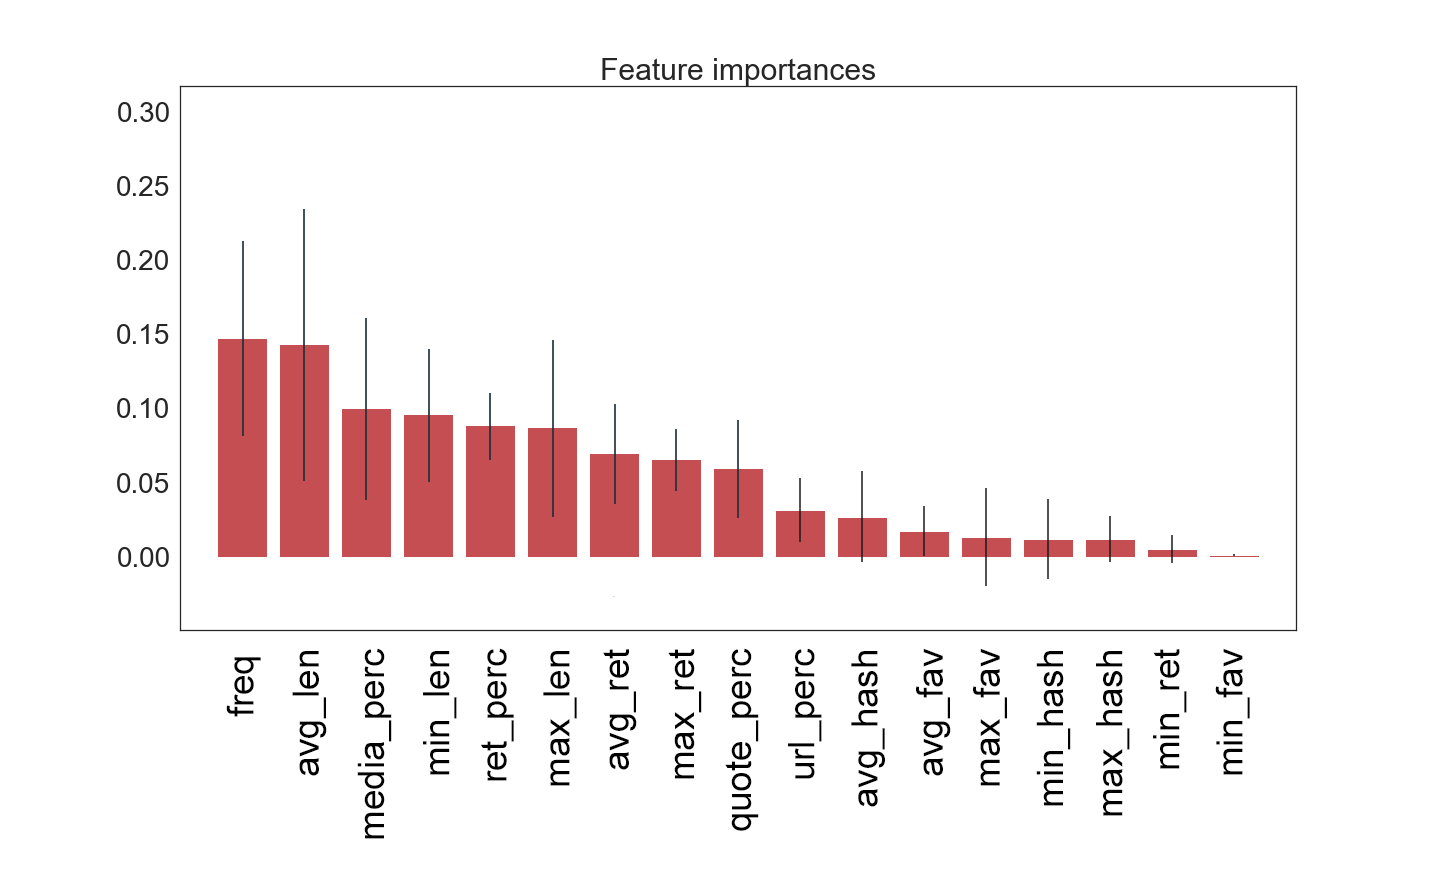
\includegraphics[width=\columnwidth]{chapter4/figure/desc_features_importances.png}
	\caption{Descriptive features ranking with Random Forest}
	\label{fig:desc_rank}
\end{figure}
As shown in Figure\ref{fig:desc_rank}, this first group has been performed a ranking function on, with the following result:\\
\textit{1. freq (0.148675), 2. avg\_len (0.140074), 3. media\_perc (0.102189), 4. min\_len (0.098582), 5. ret\_perc (0.095440), 6. max\_len (0.087577), 7. avg\_ret (0.082658), 8. max\_ret (0.063234), 9. quote\_perc (0.060392), 10. url\_perc (0.030648), 11. avg\_hash (0.030057), 12. avg\_fav (0.016788), 13. max\_fav (0.013613), 14. min\_hash (0.012777), 15. max\_hash (0.011260), 16. min\_ret (0.004959), 17. min\_fav (0.001077)}



\section{Intrinsic features}
Due the multiclass nature of our dataset, it was impossible to rely on the descriptive meta features only.

We faced the need of better capturing some behaviours, that could have helped us distinguish between targets.\\
We spent a lot of time analysing Twitter timelines by ourselves. This was one of the most useful phases of our work.\\
Indeed, we have learnt a lot about bots acting like humans on the social platform.
One thing that was easy to notice was the monotony, in terms of words or URLs involved in tweets, met with Spam-bots, as well as the opposites, for Genuine accounts or Fake-Followers.

We tried to encapsule this distinctive behaviour by adding two intrinsic features to the training vector, along with the descriptive ones.\\

How to portray such monotony?\\
We though about different approaches, like complex sentiment analysis or entity recognition, but then, we chose to rely on two methods: the TF-IDF weighting technique and the information entropy.

These two different approaches application produced two brand new features:
\small
\begin{center}
	\begin{tabular}{ll}
		\\feature&type\\
		\hline\hline
		tweet\_intradistance&float\\
		url\_entropy&float\\\hline\\
	\end{tabular}
\end{center}
\normalsize

The features were tested to fit a 

\subsection{Tweet intradistance}
We looked inside every retrieved tweets for each user, then we encoded each of them with TF-IDF weighting.\\

Every term (word) of every tweet was represented by a numeric weight, according to TF-IDF.\\
This weighting formula is a combination of Term Frequency (TF) and Inverse Document Frequency (IDF).
\[ TF_{i,j} =\frac {n_{i,j}}{|d_{j}|} \]

The term frequency factor counts the number \textit{n} of the \textit{i}\textsubscript{th} term inside the \textit{j}\textsubscript{th} document (the tweet, in our case), dividing it by the lenght of the latest, in order to give same importance to both short and long collections of texts.

\[ IDF_{i} =\log {\frac {|D|}{|\{d:i\in d\}| + 1}} \]
Where \textit{d} is the document (tweet).

The inverse document frequency factor aims to highlight the overall magnitude of the  i\textsubscript{th} term in the collection  which it belongs. The collection \textit{D}, in our work, is represented by all the gathered tweets of the examined user.
\[(TF-IDF)_{i} = TF_{i,j} \times IDF_{i} \]

After the encoding process, we wanted to map the resulting vectors into an euclidean space, in order to compute the distance of each weighted text, from the total centroid of the collection.

We decided to add each user a measure of the average intra-distance of its tweets.\\
In order to accomplish that, we relied on the WSS metric used in K-means clustering, but trying to soften its magnitude. We didn't want huge ranges in our features, minimizing the normalizations along the process.

The resulting formula for this brand new attribute is the following:
\[\textbf{tweet\_intradistance}(U) = \frac{1}{N}\sum _{\mathbf {x} \in U}\left\|\mathbf {x} -{\boldsymbol {\mu }}\right\|^{2}\]
Where \textit{N} is the number of tweet for user \textit{U}, \textit{x} is the encoded tweet and $\mu$ is the centroid of the tweet collection for that user.

This feature turned out to be pretty relevant in supporting the detections of NSFW and Spam-Bots, due their repetitive natures.

\subsection{URL entropy}

For this attribute, we decided to exploit the entropy of the information of a messages source. 
For each user U, has been computed the following:
\[\textbf{url\_entropy}(U) = \sum _{w \in W_{u}}-\frac{c(w)}{|W_{u}|}\log( \frac{c(w)}{|W_{u}|})\]
where \textit{W\textsubscript{u}} is the collection of URLs retrieved from the user's tweets. The term \textit{w} represent a single URL, belonging to the collection, and  
\textit{c(w)} is the function counting the occurrence of that URL. Finally. \textit{|W|} stands for the cardinality of the collection.

The higher the number of the different URLs inside the tweets, the higher the url\_entropy for that user.
A monotony URL spammer, with just on link in its argumentations, would lead to a zero-valued url\_entropy:
\[url\_entropy(U) = -1\log(1) = 0\]

In order to treat those URLs, we had to detect them inside the tweet texts, with some regular expressions. After the tweet was cleansed and represented only by its embedded link (if present), we wanted to handle just the domain, so we stripped all the sub-paths of the root.
We didn't care about which page or sections the bots were interested to spam, as long as the domain were the same.

\subsection{Ranking}
\begin{figure}[htp!]
	\centering
	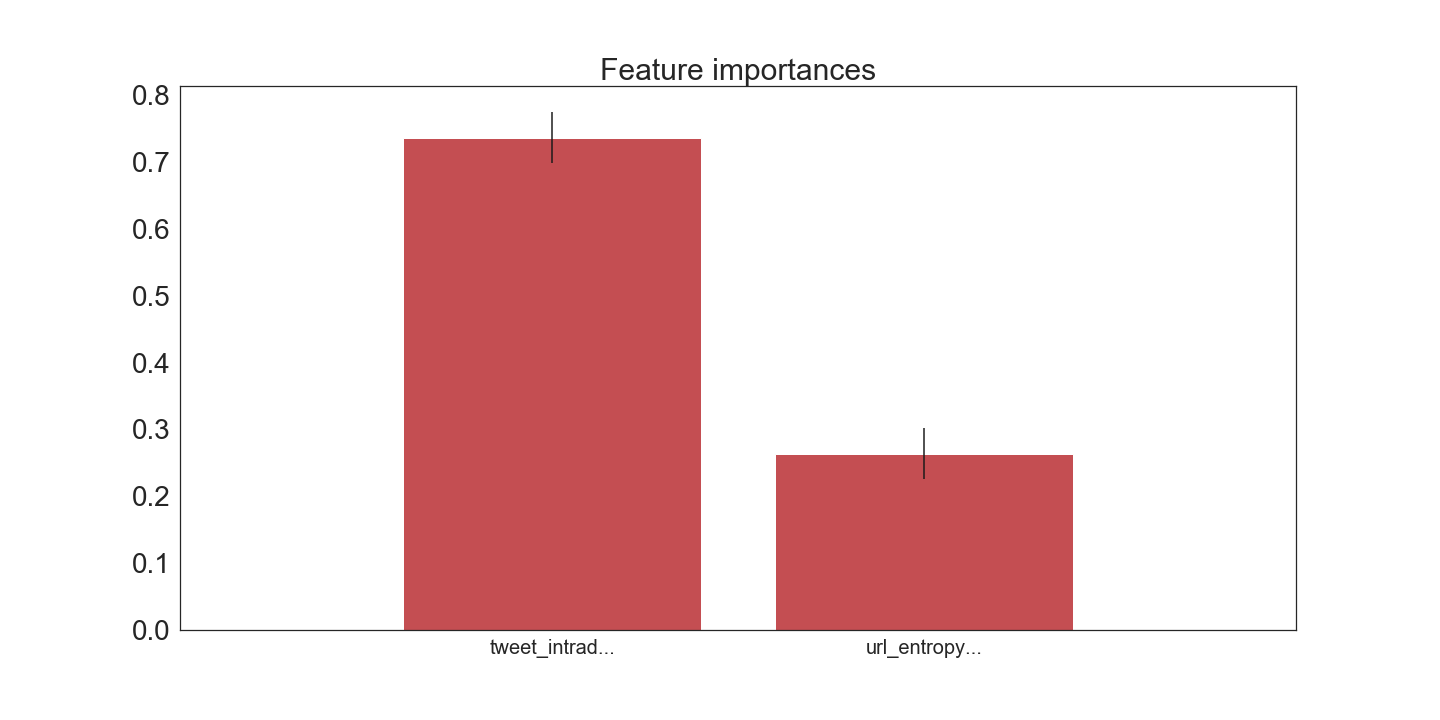
\includegraphics[width=\columnwidth]{chapter4/figure/intrinsic_features_importances.png}
	\caption{Intrinsic features ranking with Random Forest}
	\label{fig:intr_rank}
\end{figure}
Figure\ref{fig:intr_rank} shows the inner ranking of these two new features, that have these scores:
\textit{1. tweet\_intradistance (0.736293), 2. url\_entropy (0.263707)}
\section{Extrinsic features}
Once we have modelled the personal twitting actions, in terms of words and links dissimilarity, we needed to look for those parameters that could be compared with all the users in our dataset.
We wanted the users to get out of their shells, and to match their timelines with each others.

Once again, sentiment analysis came to our mind. We found lots of paid or limited services that could have only partially supported us during this stage.
We couldn't think about implementing our own semantic analysis, as it is meant to be, due to the effort and time it would had taken.
For simplicity sake, we had the idea to look for the most meaningful words in tweets, that are common to all the users belonging to the same class.
We tried this approach, hoping to find a robust help in separating topics among targets.

The idea was to build various partially-non-overlapping dictionaries, one for each class of users, containing the most popular words used by them in their retrieved tweets, stripped of stopwords. Each dictionary is ordered according to the occurrence of each word, in order to have a proper ranking for the terms and to give each of them a score.
The magnitude of the non-overlapping portions of these lists will be shown soon, in this section.

We gathered the 1000 most common words for each category of accounts.

\subsection{Scores computation}

\subsubsection{Multiclass Dataset}
After the dictionaries related to the multiclass dataset were filtered, to prevent (partial) overlapping, we had four collections, composed by the tuples \textit{(word, score)}:
\small
\begin{center}
	\begin{tabular}{ll}
		\\dictionary&size\\
		\hline\hline
		NSFW\_main\_words.csv&253\\
		news\_spreders\_main\_words.csv&424\\
		spam\_bots\_main\_words.csv&325\\
		fake\_followers\_main\_words.csv&469\\\hline\\
	\end{tabular}
\end{center}
\normalsize

The overall scores are normalized, so that the most common word, for each class, is associated with a unitary weight, the least common one with a value similar to zero (it depends on the final amount of words included in the dictionary).

In terms of representation, this \textit{keywords score} is built with 4 different values, one for each class.\\

If some user hit a word that is placed inside more than a dictionary, we wanted to let the relative weights speak and assign scores to each of the targets that contain that word, knowing they are less relevant, as they don't fall in the highest positions.\\
So we have

\small
\begin{center}
	\begin{tabular}{ll}
		\\feature&type\\
		\hline\hline
		NSFW\_words\_score&float\\
		spam\_bots\_words\_score&float\\
		news\_spreders\_words\_score&float\\
		fake\_followers\_words\_score&float\\\hline\\
	\end{tabular}
\end{center}
\normalsize
When we process a new user and infer on him, we scan every words of every tweets and match them with all the dictionary. Every time that we hit a listed word, we assign the user the score of that word.

For instance, If the word we are comparing matches with the most frequent for NSFW accounts (the top position in its dictionary), we update the \textit{NSFW\_words\_score} of our user, summing 1 to its current value for that feature.

The followings are examples of the top three words used by our bot categories:
\small
\begin{center}
	\begin{tabular}{lllll}
		\multicolumn{5}{c}{\textbf{NSFW dictionary}} \\
		\hline\hline
		\multicolumn{4}{l}{\textit{word}} & 
		\multicolumn{1}{r}{\textit{score}}\\
		\hline\hline
		\multicolumn{4}{l}{bio} & 
		\multicolumn{1}{r}{1.000}\\
		\multicolumn{4}{l}{photos} & 
		\multicolumn{1}{r}{0.167}\\
		\multicolumn{4}{l}{p$ \dot{a} $} & 
		\multicolumn{1}{r}{0.160}\\
		\multicolumn{5}{c}{...} \\
		\hline\\
	\end{tabular}
\end{center}
\normalsize
\small
\begin{center}
	\begin{tabular}{lllll}
		\multicolumn{5}{c}{\textbf{News-Spreader dictionary}} \\
		\hline\hline
		\multicolumn{4}{l}{\textit{word}} & 
		\multicolumn{1}{r}{\textit{score}}\\
		\hline\hline
		\multicolumn{4}{l}{obama} & 
		\multicolumn{1}{r}{1.000}\\
		\multicolumn{4}{l}{g7} & 
		\multicolumn{1}{r}{0.723}\\
		\multicolumn{4}{l}{potus} & 
		\multicolumn{1}{r}{0.690}\\
		\multicolumn{5}{c}{...} \\
		\hline\\
	\end{tabular}
\end{center}
\normalsize
\small
\begin{center}
	\begin{tabular}{lllll}
		\multicolumn{5}{c}{\textbf{Spam-Bots dictionary}} \\
		\hline\hline
		\multicolumn{4}{l}{\textit{word}} & 
		\multicolumn{1}{r}{\textit{score}}\\
		\hline\hline
		\multicolumn{4}{l}{talnts} & 
		\multicolumn{1}{r}{1.000}\\
		\multicolumn{4}{l}{developer} & 
		\multicolumn{1}{r}{0.511}\\
		\multicolumn{4}{l}{engineer} & 
		\multicolumn{1}{r}{0.467}\\
		\multicolumn{5}{c}{...} \\
		\hline\\
	\end{tabular}
\end{center}
\normalsize
\small
\begin{center}
	\begin{tabular}{lllll}
		\multicolumn{5}{c}{\textbf{Fake-Followers dictionary}} \\
		\hline\hline
		\multicolumn{4}{l}{\textit{word}} & 
		\multicolumn{1}{r}{\textit{score}}\\
		\hline\hline
		\multicolumn{4}{l}{iPhone} & 
		\multicolumn{1}{r}{1.000}\\
		\multicolumn{4}{l}{cheap} & 
		\multicolumn{1}{r}{0.993}\\
		\multicolumn{4}{l}{bounty} & 
		\multicolumn{1}{r}{0.856}\\
		\multicolumn{5}{c}{...} \\
		\hline\\
	\end{tabular}
\end{center}
\normalsize

We expected to capture patterns about the choice of the words involved in tweets, for each of our categories.
This extrinsic attributes revealed themselves as very useful, lately.

\subsubsection{Binary Dataset}
As for the Multiclass dataset, we computed two dictioraries based on the Binary dataset classes.

\small
\begin{center}
	\begin{tabular}{ll}
		\\dictionary&size\\
		\hline\hline
		bots\_main\_words.csv&315\\
		genuine\_followers\_main\_words.csv&315\\\hline\\
	\end{tabular}
\end{center}
\normalsize

The result seemed to be acceptable for the bot dictionary, while the genuine one contains many non-english words. The top three words (with their scores) for both dictionaries are:

\small
\begin{center}
	\begin{tabular}{lllll}
		\multicolumn{5}{c}{\textbf{bot dictionary}} \\
		\hline\hline
		\multicolumn{4}{l}{\textit{word}} & 
		\multicolumn{1}{r}{\textit{score}}\\
		\hline\hline
		\multicolumn{4}{l}{weight} & 
		\multicolumn{1}{r}{1.000}\\
		\multicolumn{4}{l}{loss} & 
		\multicolumn{1}{r}{0.744}\\
		\multicolumn{4}{l}{traffic} & 
		\multicolumn{1}{r}{0.661}\\
		\multicolumn{5}{c}{...} \\
		\hline\\
	\end{tabular}
\end{center}
\normalsize

\small
\begin{center}
	\begin{tabular}{lllll}
		\multicolumn{5}{c}{\textbf{genuine dictionary}} \\
		\hline\hline
		\multicolumn{4}{l}{\textit{word}} & 
		\multicolumn{1}{r}{\textit{score}}\\
		\hline\hline
		\multicolumn{4}{l}{nao} & 
		\multicolumn{1}{r}{1.000}\\
		\multicolumn{4}{l}{pra} & 
		\multicolumn{1}{r}{0.563}\\
		\multicolumn{4}{l}{uma} & 
		\multicolumn{1}{r}{0.493}\\
		\multicolumn{5}{c}{...} \\
		\hline\\
	\end{tabular}
\end{center}
\normalsize

\subsection{Safe Area}
Making a step back, before the overall computation of this group of features, we had to decide the portions of the dictionaries that weren't supposed to overlap with each others.
Once we gathered the main words for each bot class, we had to chose ths size of what we called the \textit{Safe Area}.
The Safe Area is the collection of the first N words, in each dictionary, that are not overlapping with the others listed in the other dictionaries.
This method has been applied to ensure that some words resulted as strictly category-characterizing.
We had to pick the number of the top N words that had to be representing, for each category.

We tried with four different portions of the collections: the 25\% of the words, the 50\%, the 75\% and the total non-overlapping solution, the 100\% of the terms.

We computed four different dataset (starting from the multiclass collection), one for each parameter, and tested the outcomes of this process on them. The testing phase was composed by the features ranking, like done before, but considering the whole feature vector, and by a \textit{10-fold-crossvalidation} scoring. This last technique has been widely used during all our work, and will be explained in details in the following chapter.
Figures \ref{fig:250_overall} and \ref{fig:250_closeup} list the results for the  first tested Safe Area, with 250 words involved in that zone, and the dictionaries that are overlapping for the 75\%. The following Figures \ref{fig:500_overall}, \ref{fig:500_closeup} represent the situation with half of the words included in the Safe Areas. So do Figures \ref{fig:750_overall} and \ref{fig:750_closeup}, with the 75\% of the safe terms, and, finally, Figures \ref{fig:1000_overall} and \ref{fig:1000_closeup}, with totally disjointed dictionaries.

Looking at these graphics, we could infer that the most meaningful feature, for the Random Forest, had been computed with the score of the NSFW\_words list.
The overall placements in the rankings are similar among the different datasets.
\begin{itemize}
	\item[\PencilRight]250 words in the Safe Area - overall ranking placement:\\
	\textbf{8.} news\_spreaders\_words\_score, \textbf{10.} NSFW\_words\_score, \textbf{16.} spam\_bots\_words\_score, \textbf{20.} fake\_followers\_words\_score.
	
	\item[\PencilRight]500 words in the Safe Area - overall ranking placement:\\
	\textbf{7.} news\_spreaders\_words\_score, \textbf{9.} NSFW\_words\_score, \textbf{13.} spam\_bots\_words\_score, \textbf{22.} fake\_followers\_words\_score.
	
	\item[\PencilRight]750 words in the Safe Area - overall ranking placement\\
	\textbf{8.} news\_spreaders\_words\_score, \textbf{12.} NSFW\_words\_score, \textbf{13.} spam\_bots\_words\_score, \textbf{24.} fake\_followers\_words\_score.
	
	\item[\PencilRight]100 words in the Safe Area (disjointed lists) - overall ranking placement:\\
	\textbf{8.} news\_spreaders\_words\_score, \textbf{11.} NSFW\_words\_score, \textbf{14.} spam\_bots\_words\_score, \textbf{25.} fake\_followers\_words\_score.
\end{itemize}

We needed another confrontation term, which could tell us something about the goodness of the classifier, in relation with the number of safe words used for the computation of the features.
We validated a Random Forest multiclass classifier, with increasing number of trees in the forest. Figure \ref{fig:safe_areas} shows the results.

\begin{figure}[htp!]
	\centering
	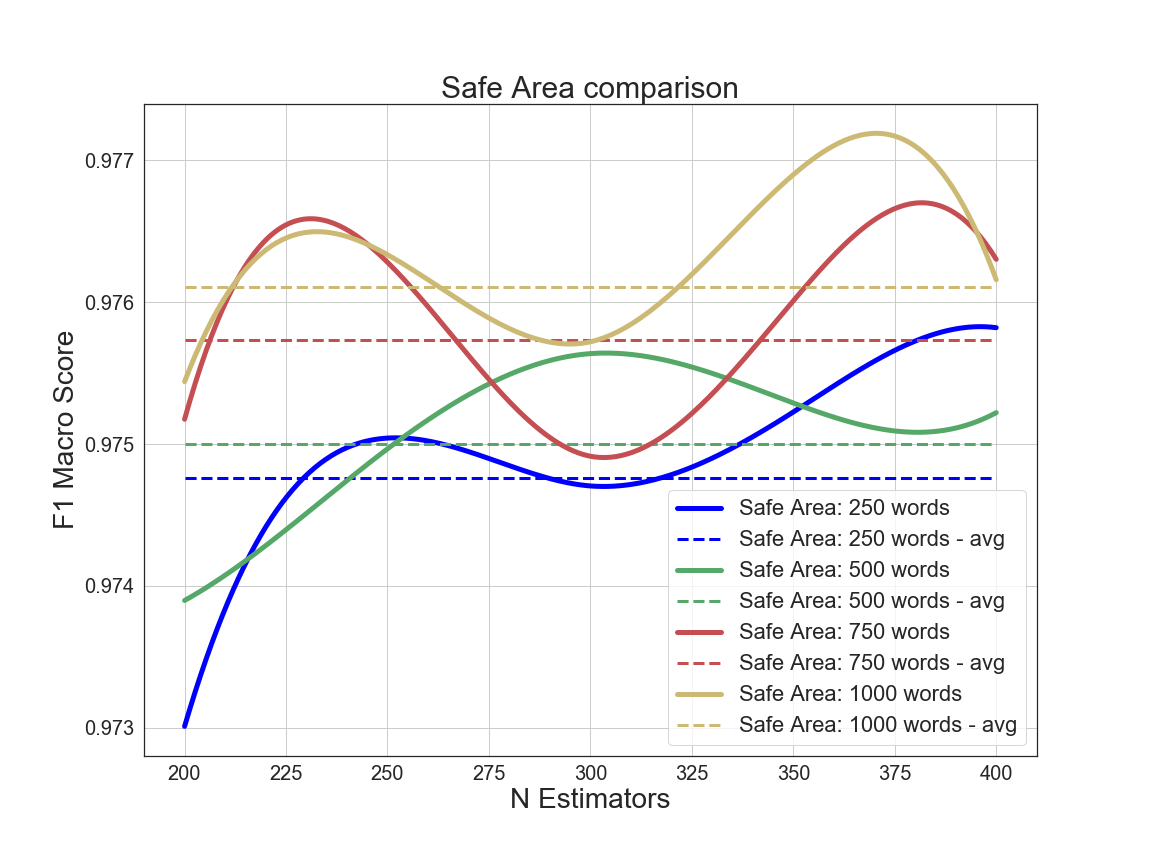
\includegraphics[width=\columnwidth]{chapter4/figure/dict_comparison.png}
	\caption{Safe Areas comparison}
	\label{fig:safe_areas}
\end{figure}

The best looking number of words to save was 1000. The totally non-overlapping solution would have provided us the best F1 score, once we would have started developing the final models. We decided to go with that configuration to build the extrinsic features. 

\begin{figure}[htp!]
	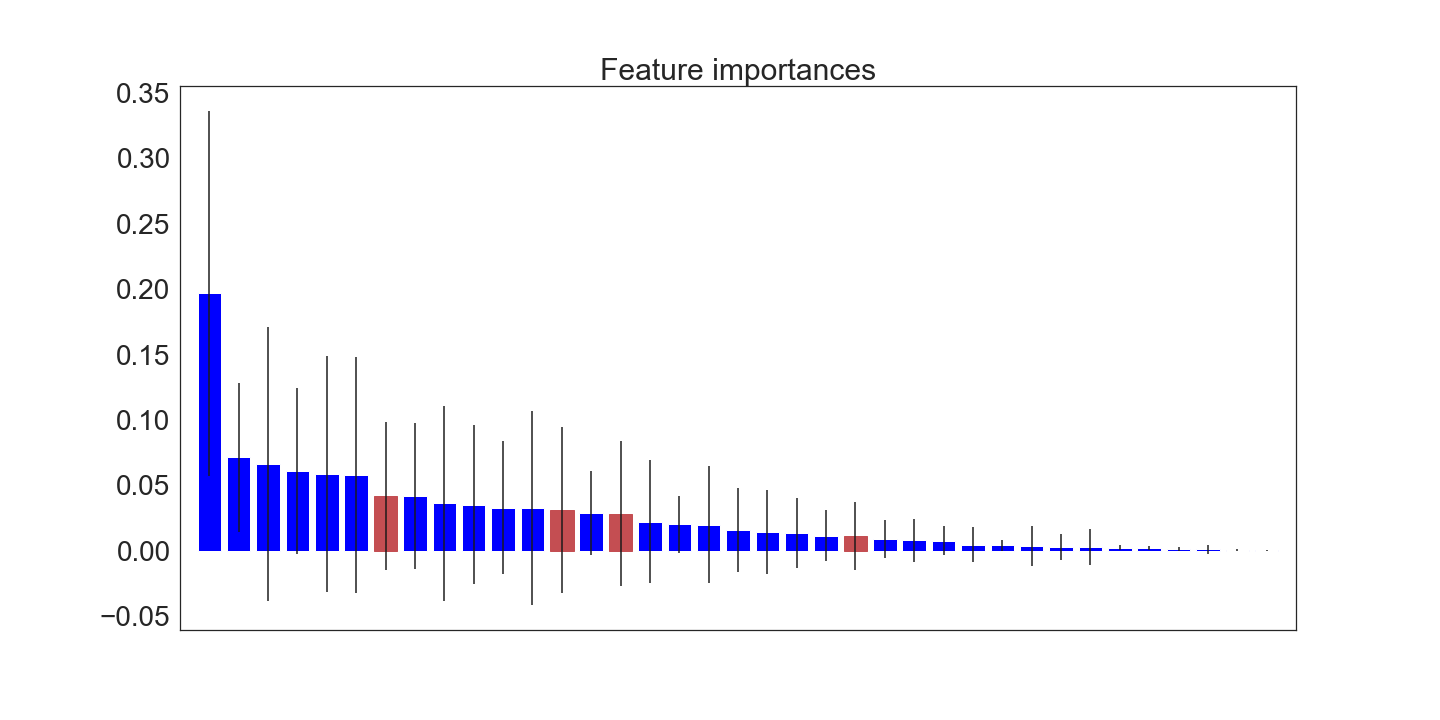
\includegraphics[width=\columnwidth]{chapter4/figure/features_importances_250.png}
	\caption{Features ranking - Safe Area = 250}
	\label{fig:250_overall}
\end{figure}
\begin{figure}[htp!]
	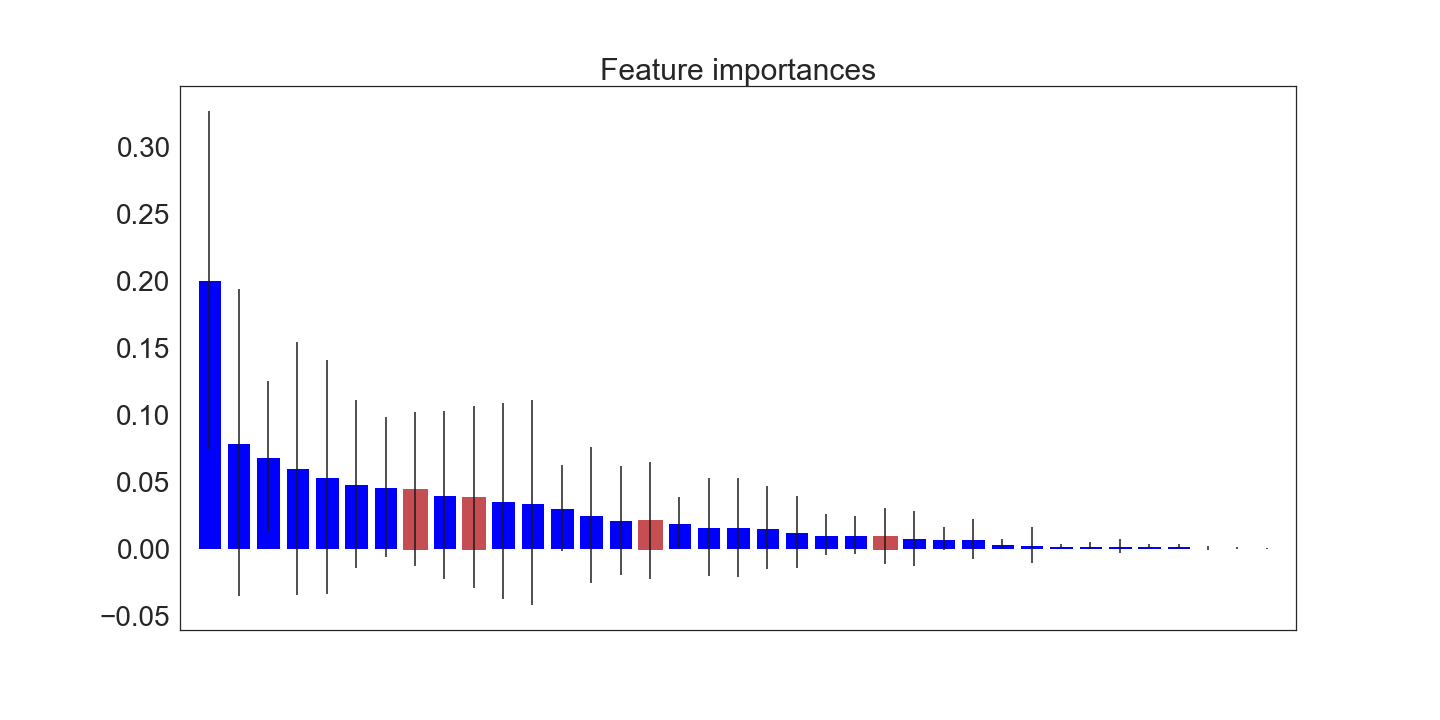
\includegraphics[width=\columnwidth]{chapter4/figure/features_importances_500.png}
	\caption{Features ranking - Safe Area = 500}
	\label{fig:500_overall}
\end{figure}
\begin{figure}[htp!]
	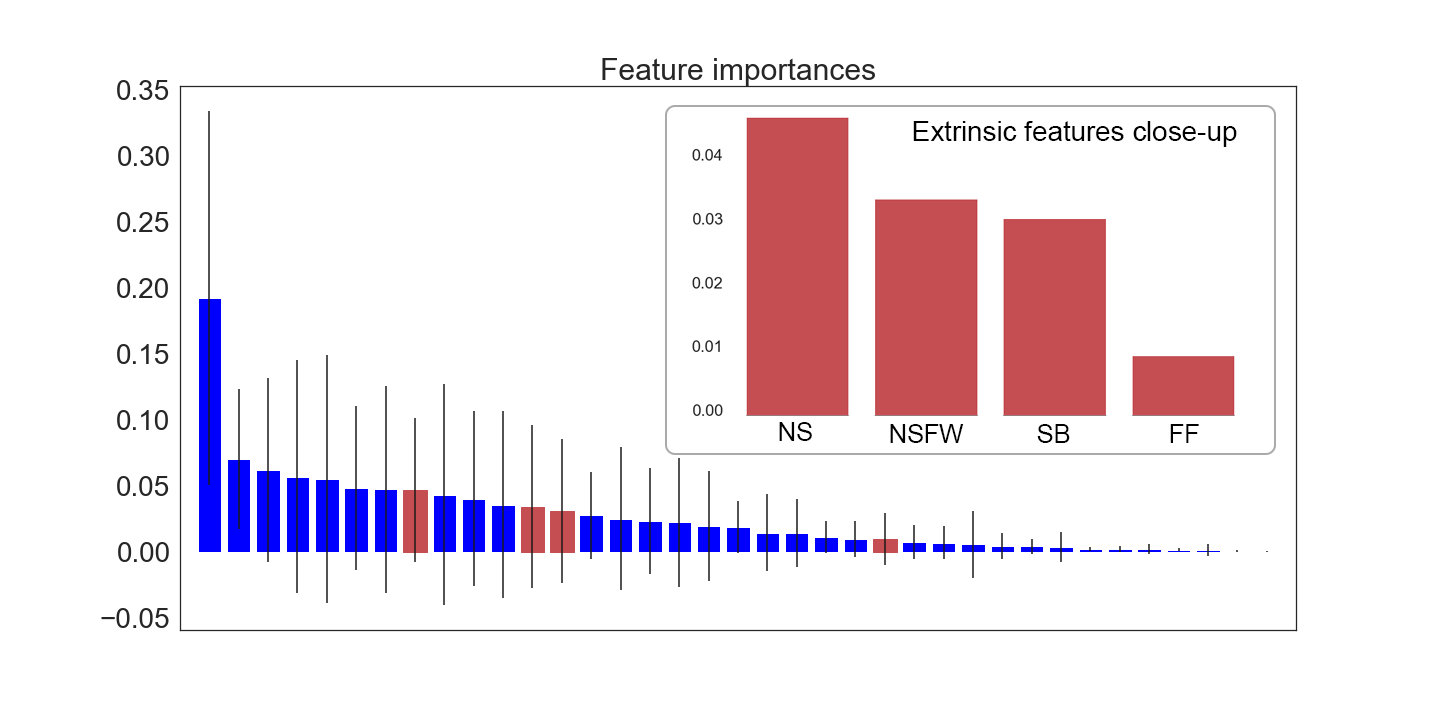
\includegraphics[width=\columnwidth]{chapter4/figure/features_importances_750.png}
	\caption{Features ranking - Safe Area = 750}
	\label{fig:750_overall}
\end{figure}
\begin{figure}[htp!]
	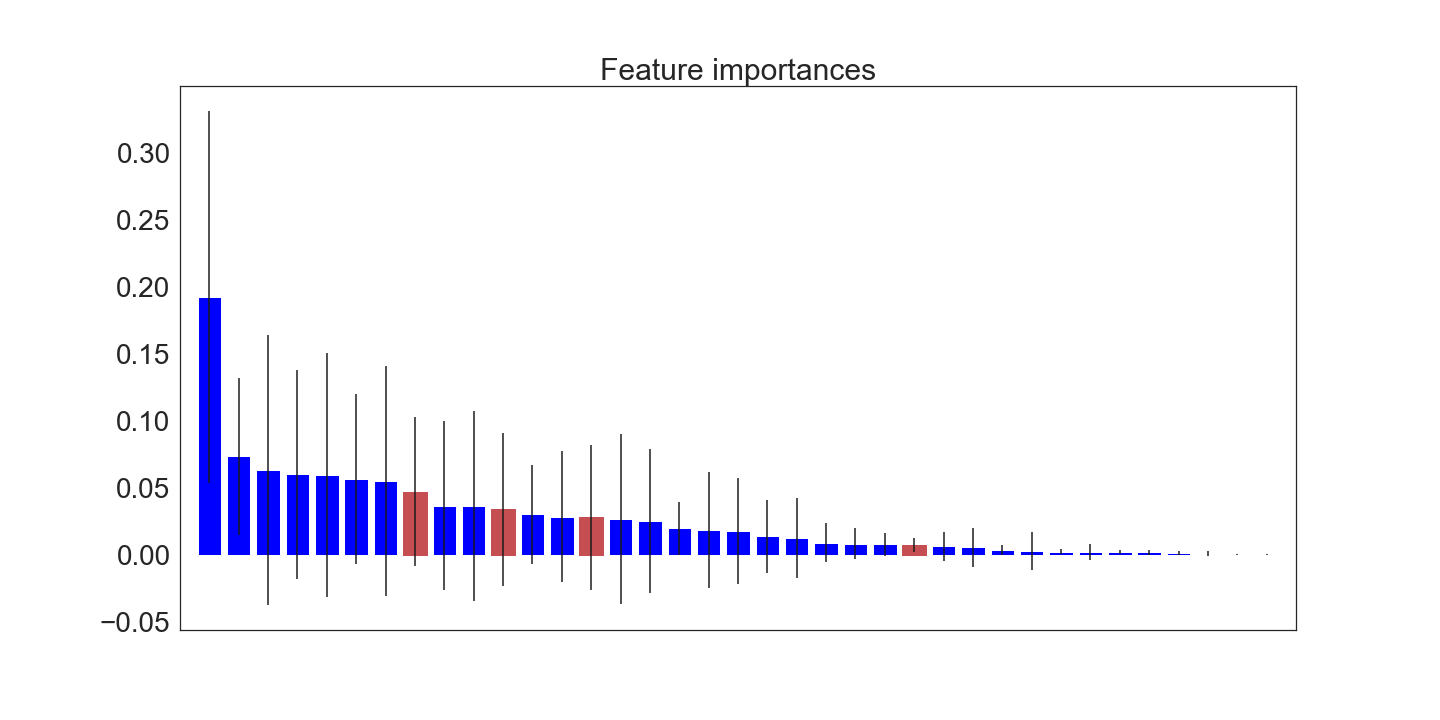
\includegraphics[width=\columnwidth]{chapter4/figure/features_importances_1000.png}
	\caption{Features ranking - Safe Area = 1000}
	\label{fig:1000_overall}
\end{figure}


\section{Image features}
One of the main issues of our work was to make the NSFW class different, in terms of classifiers vision, with respect of Spam-bots.

According to our user-based, descriptive and intrinsic features, both classes act in a similar way: they spam similar links, have high tweet frequency and their contents are often repeated.\\
What could be the difference?

We started with "blind" classifier, that was the main problem. Our feature vector lacked in visual components. A Spam-bot could have been detected as a NSFW, as its tweets involved media and URLs. We needed to go deep and actually see what kind of media were broadcast.
This is the reason for presence of the upcoming features.

We've found a small versatile project on GitHub for NSFW detection.\\
The projects involves a pre-trained TensorFlow neural network for image recognition, that looks for adult and violent content inside pictures. It assigns the media a probability to be not safe for work.

The model exploits the Inception v3 \cite{inception} architecture.
It takes a 299x299x3 input, representing a 299 pixels squared visual field and 3 color channels (R,G,B). It has five convolutional layers, with two max-pooling operations between them. Successively, it stacks multiple "Inception modules" and it ends with a softmax output layer.
The repeated stacking of such models makes the architecture much deep, allowing each module to detect features on multiple scales, using convolution operations with different kernel sizes.


The Inception model has been fed with pictures representing Not Safe For Work contents, as well as Safe For Work contents.
The NSFW images has been retrieve by crawling the browser tabs, with the help of Fatkun batch download Images, a Google Chrome extension for batch downloads.
We gathered 1,548 elements for that class.
The SFW class content is composed by a collection of clean pictures of random users, already collected in the Selfie Dataset \cite{selfie} . This dataset contains 46,836 images, wiht metadata about genders, ages and so on; it's built for research purposes.
We just randomly picked the same number as for the other class, in order to have a balanced training set.

The network has then been trained with 500 iteration steps, leading to a  95.7\% of accuracy in validation and 99\% in training stage, when distinguish nsfw contents from sfw ones. The accuracy graph is shown in Figure \ref{fig:inception}.
We thought that the bias introduced with this new features would have been under control and that it wouldn't compromise the final results of our models.

\begin{figure}[htp!]
	\centering
	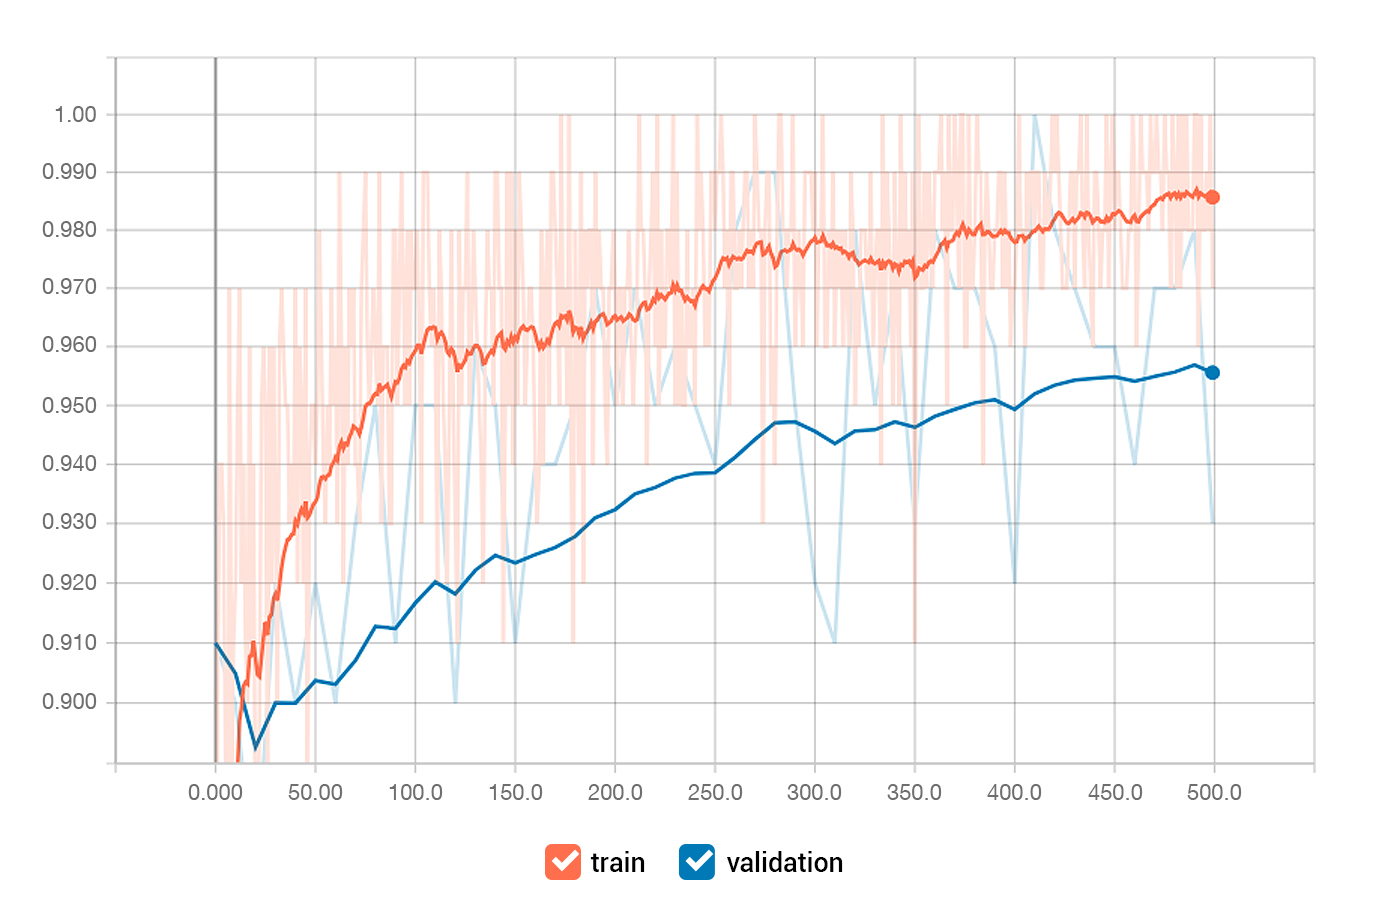
\includegraphics[width=\columnwidth]{chapter4/figure/inception.jpg}
	\caption{Train and validation accuracy through learning steps}
	\label{fig:inception}
\end{figure}

We decided to scan our dataset with this new component and to give a NSFW score to both profile pictures and tweets.
For time complexity reasons, we couldn't imagine to scan all the retrieved tweets for each user and to look for embedded media. We limited the process to the latest ten tweets.

Obviously, the prediction time has been affected by this new preprocessing stage, but we think that this number of pictures analysed (up to eleven), makes the generalization duration still reasonable.

The brand new attributes that helped us in better separating NSFW class are:
\small
\begin{center}
	\begin{tabular}{ll}
		\\feature&type\\
		\hline\hline
		NSFW\_profile&float\\
		NSFW\_avg&float\\\hline
	\end{tabular}
\end{center}
\normalsize

\section{Final feature vectors}
\label{sec:feature_vector}

\subsection{Multiclass Dataset}
At the end of this process we obtained a feature vector composed of 37 elements, 12 based on the user and 26 based on his tweets.

\subsubsection{User features}


\small
\begin{center}
	\begin{tabular}{lll}
		\textbf{Features}\\
		\hline\hline
		age\\
		default\_profile\\
		description\_len\\
		favourites\_count\\
		friends\_count\\
		followers\_count\\
		listed\_count\\
		profile\_use\_background\_image\\
		name\_len\\
		screen\_name\_len\\
		statuses\_count\\
		url\\
		\hline\\
		
	\end{tabular}
\end{center}
\normalsize

\subsubsection{Tweets features}
\small
\begin{center}
	\begin{tabular}{lll}
		\textbf{Descriptive features}\\
		\hline\hline
		freq\\
		min\_fav\\
		avg\_fav\\
		max\_fav\\
		min\_hash\\
		avg\_hash\\
		max\_hash\\
		min\_len\\
		avg\_len\\
		max\_len\\
		min\_ret\\
		avg\_ret\\
		max\_ret\\
		media\_perc\\
		quote\_perc\\
		ret\_perc\\
		url\_perc\\\hline\\
	\end{tabular}
\end{center}

\begin{center}
	\begin{tabular}{lll}
		\textbf{Intrinsic features}\\
		\hline\hline
		tweets\_intradistance\\
		url\_intradistance\\\hline\\
	\end{tabular}
\end{center}


\begin{center}
	\begin{tabular}{lll}
		\textbf{Extrinsic features}\\
		\hline\hline
		NSFW\_words\_score\\
		news\_spreaders\_words\_score\\
		spam\_bots\_words\_score\\
		fake\_followers\_words\_score\\
		\hline\\
	\end{tabular}
\end{center}

\begin{center}
	\begin{tabular}{lll}
		\textbf{Images features}\\
		\hline\hline
		NSFW\_profile\\
		NSFW\_avg\\\hline\\
	\end{tabular}
\end{center}

\normalsize

\subsection{Binary Dataset}
At the end of this process we obtained a feature vector composed of 33 elements, 12 based on the user and 21 based on his tweets.

\subsubsection{User features}


\small
\begin{center}
	\begin{tabular}{lll}
		\textbf{Features}\\
		\hline\hline
		default\_profile\\
		description\_len\\
		favourites\_count\\
		friends\_count\\
		followers\_count\\
		listed\_count\\
		profile\_use\_background\_image\\
		name\_len\\
		screen\_name\_len\\
		statuses\_count\\
		url\\
		verified\\
		\hline\\
		
	\end{tabular}
\end{center}
\normalsize

\subsubsection{Tweets features}
\small
\begin{center}
	\begin{tabular}{lll}
		\textbf{Descriptive features}\\
		\hline\hline
		freq\\
		min\_fav\\
		avg\_fav\\
		max\_fav\\
		min\_hash\\
		avg\_hash\\
		max\_hash\\
		min\_len\\
		avg\_len\\
		max\_len\\
		min\_ret\\
		avg\_ret\\
		max\_ret\\
		media\_perc\\
		quote\_perc\\
		ret\_perc\\
		url\_perc\\\hline\\
	\end{tabular}
\end{center}

\begin{center}
	\begin{tabular}{lll}
		\textbf{Intrinsic features}\\
		\hline\hline
		tweets\_intradistance\\
		url\_intradistance\\\hline\\
	\end{tabular}
\end{center}


\begin{center}
	\begin{tabular}{lll}
		\textbf{Extrinsic features}\\
		\hline\hline
		bots\_words\_score\\
		genuine\_words\_score\\
		\hline\\
	\end{tabular}
\end{center}

\normalsize
